\graphicspath{{./Annexe_capacites_segm/images/}}

\chapter{Efficacité et robustesse de l'algorithme de segmentation}
\label{annexe:capacites_segm}

Dans le but d'étudier l'efficacité et les limites de l'algorithme de segmentation, des essais ont été menés sur des échantillons créés de toute pièce. L'échantillon est un empilement de sphères parfaites en contact. La géométrie parfaite permet de quantifier certaines propriétés du milieu ainsi produit (comme sa densité). La forme sphérique permet de travailler sur des éléments courbés vis-à-vis de la géométrie des voxels constituant l'image et d'établir des zones de contact relativement petites en surface. De manière à travailler sur un échantillon dont le nombre de particules est de l'ordre de grandeur de celui des images de tomographie traitées pour la segmentation, l'échantillon comporte un total de \num{100} sphères dont l'écart maximal en volume est de $16\%$. \'Etant donné la géométrie cubique des voxels, il s'avère impossible de générer des sphères parfaites dans une image. On peut cependant générer des sphères quasi-parfaites en considérant la part du volume de chaque voxel dans le volume de la sphère pour déterminer la valeur de ce voxel. L'outil Kalisphera \citep{tengattini_kalisphera_2015} permet de faire cela et a été utilisé dans cet objectif.
\\Les rayons des sphères et leur agencement étant connus, il est possible d'extraire des informations du milieu granulaire ainsi créé. Calculer ces mêmes informations après segmentation et les comparer avec celles de l'image d'origine permet alors de déterminer l'efficacité de l'algorithme. En ce qui concerne la robustesse, il a été vu en détail dans la partie précédente la capacité de l'algorithme à segmenter des particules dont les formes sont très hétérogènes et complexes. Un gros effort a été fourni afin de permettre cela et, au vue des comparaisons entre les reconstructions tomographiques et les volumes segmentés, l'objectif de segmenter ce type de particules est validé. Il peut en outre être intéressant d'observer les capacités de l'algorithme à segmenter des volumes dont le bruit et le flou des images sont relativement élevés. Pour cela, l'image créée artificiellement est soumise à différentes fonctions de bruitage et floutage afin de simuler un signal issu d'expérimentations dont le bruit et le flou sont relativement plus élevés que sur les reconstructions de tomographies observées dans cette thèse. Si la segmentation réussit, alors l'algorithme est suffisamment robuste pour traiter les images expérimentales.
\\Les effets du floutage et du bruitage sont observables sur la figure \ref{fig05:spheres_bruitage}. L'image d'origine subit, dans l'ordre, les traitements suivants :
\begin{itemize}
	\item un flou gaussien 3D dont l'écart-type est de $1$ ;
	\item un bruit aléatoire dont la distribution est une gaussienne de moyenne $0$ et d'écart-type $55$ ;
	\item un second flou gaussien dont l'écart-type est de $1$ ;
	\item un second bruit aléatoire de distribution normale dont l'écart-type est de $10$.
\end{itemize}
L'analyse des histogrammes sur la figure \ref{fig05:spheres_bruitage} indique bien un rapprochement du signal de sortie avec celui des images issues de la tomographie (cf. figure \ref{fig04:contrast_enhancement_filtering}).
\begin{figure}\centering
	\subfloat[Image créée à partir de l'outil Kalisphera]{
		\includegraphics[height=0.3\textwidth]{benchmark/original.jpg}\hspace{0.5cm}
		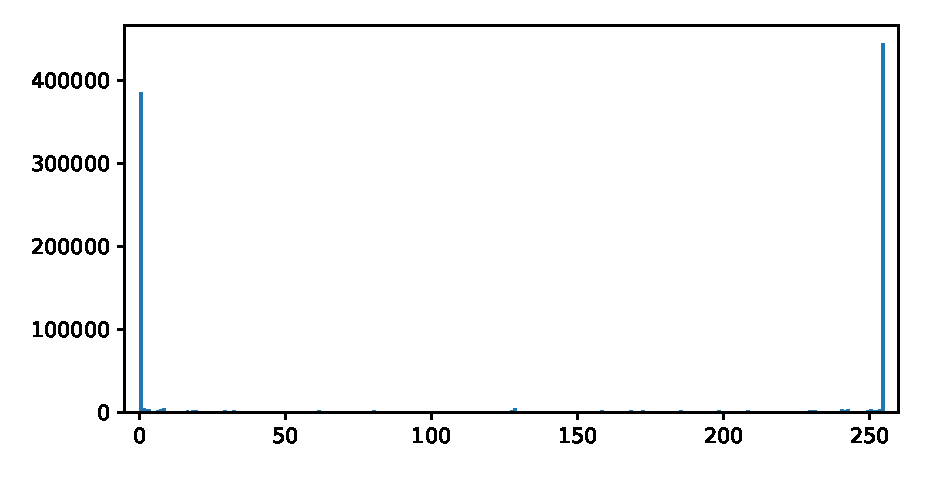
\includegraphics[height=0.3\textwidth]{benchmark/histogram_orig.eps}}\\
	\subfloat[Image bruitée artificiellement]{
		\includegraphics[height=0.3\textwidth]{benchmark/noised.jpg}\hspace{0.5cm}
		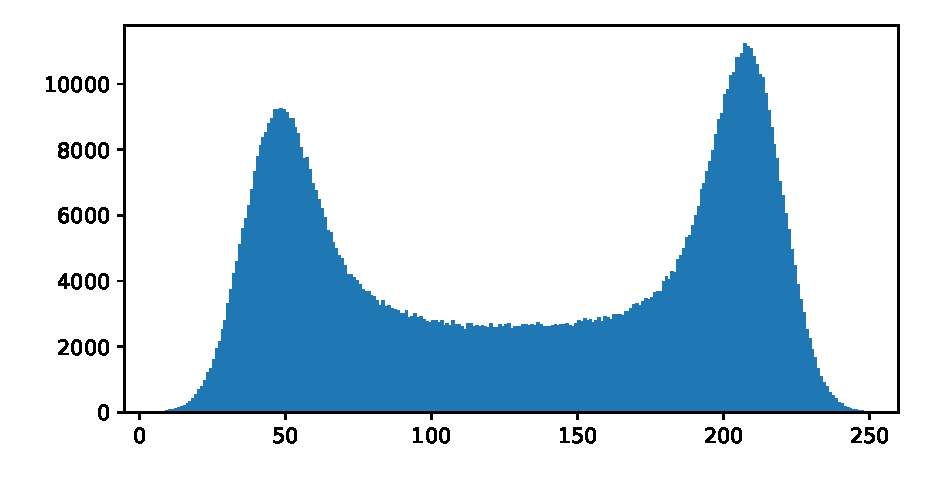
\includegraphics[height=0.3\textwidth]{benchmark/histogram_noised.eps}}
	\caption{\label{fig05:spheres_bruitage}Coupes 2D et histogrammes des images (a) d'origine et (b) bruitée artificiellement}
\end{figure}
\\L'objectif est d'observer les résultats de la segmentation lorsque l'image artificiellement bruitée est donnée en entrée du script de segmentation. Ces résultats sont visibles sur la figure \ref{fig05:3D_spheres_segmentation} dans laquelle on distingue les vues 3D du volume d'origine et du volume segmenté, mais aussi des histogrammes. Ces histogrammes représentent le nombre de sphères ayant un volume donné. Le volume considéré ici est le volume normalisé : pour une sphère donnée, il s'agit du ratio du volume de la sphère et du volume total de l'image 3D. La discrétisation de l'histogramme du volume d'origine se retrouve sur l'image segmentée, bien que chaque valeur discrète soit plus étendue. Pour une taille de sphère donnée, les volumes des sphères ne sont plus exactement les mêmes : la géométrie n'est plus parfaite. Cela vient très probablement de l'ajout du bruit artificiel, d'erreurs liées au seuillage mais aussi de la définition des frontières lors de la segmentation. De même, il est remarqué un léger décalage du signal qui s'accentue vers les sphères les plus volumineuses. Ce décalage illustre le fait que les sphères issues de la segmentation ont un plus grand volume que celles de l'image d'origine. Puisque cet effet évolue de pair avec la surface des sphères, il est constaté une corrélation entre l'erreur existante et une mauvaise définition de la frontière des particules. Les vues 3D de la figure \ref{fig05:3D_spheres_segmentation} montrent malgré tout un résultat très convaincant et le fait que la discrétisation du signal soit conservée indique que l'information sur le milieu l'est également. Afin de quantifier cette erreur, une analyse des densités apparentes des milieux représentés est faite. Le tableau \ref{tab05:d_bulk_benchmark} rend compte des résultats : les trois valeurs indiquées sont, dans l'ordre de lecture, la densité calculée théoriquement à partir de la définition de l'agencement des sphères, celle mesurée sur l'image produite par Kalisphera (donc voxellisée) et celle mesurée à partir de l'image dégradée puis segmentée. La mesure de la densité apparente sur une image représentant un milieu granulaire correspond au ratio du nombre de voxels représentant les grains et du nombre de voxels total dans l'image. La densité théorique de l'agencement a été calculée en additionnant les volumes exacts des sphères et en divisant la somme par le plus petit cube qui contient l'ensemble des grains. De nouveau, le constat d'une augmentation du volume des sphères lors de la segmentation est fait. L'écart relatif sur la mesure de densité entre le volume dégradé puis segmenté et le volume théorique est de \SI{2.8}{\percent}. Compte tenu de la quantité de bruit et de la qualité du signal du volume artificiellement dégradé, ce résultat est positif et vient confirmer la capacité du script à segmenter des images 3D de milieux granulaires complexes, même pour des images de faible qualité.
\begin{figure}\centering
	\subfloat[Volume d'origine]{
		\includegraphics[width=0.4\textwidth]{benchmark/original_3D_rescale.png}}\hspace{5em}
	\subfloat[Volume segmenté]{
		\includegraphics[width=0.4\textwidth]{benchmark/segm_3D_rescale.png}}\\
	\subfloat[Histogramme des volumes normalisés pour l'image d'origine]{
		\includegraphics[width=\textwidth]{benchmark/histogram_volume_real.eps}}\\
	\subfloat[Histogramme des volumes normalisés pour l'image segmentée]{
		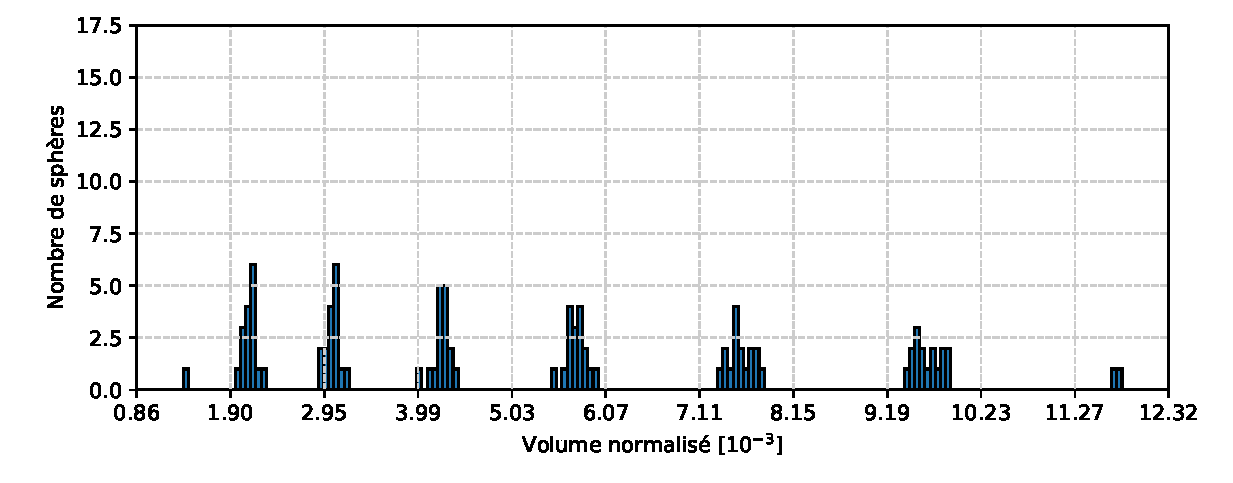
\includegraphics[width=\textwidth]{benchmark/histogram_volume_segm.eps}}
	\caption{\label{fig05:3D_spheres_segmentation}Résultats de la segmentation 3D sur l'échantillon de 100 sphères}
\end{figure}
\begin{table}\centering
	\begin{tabular}{c@{  \textbullet\  }c@{  \textbullet\  }c}
		\hline
		\multicolumn{3}{c}{Densités apparentes des milieux représentés par :}\\
		l'agencement initial & le volume d'origine & le volume segmenté \\\hline
		$0.533$ & $0.531$ & $0.548$\\\hline
	\end{tabular}
	\caption{\label{tab05:d_bulk_benchmark}Densités apparentes mesurées sur les images de tests}
\end{table}
\\L'ensemble des résultats présentés dans cette partie permet de rendre compte de l'efficacité et de la robustesse de l'algorithme de segmentation. En effet, en plus du fait que l'algorithme est basé sur une méthode de segmentation des grains à géométrie complexe, il semble également adapté aux images expérimentales dont le signal est relativement bruité. Il a été également vu que l'algorithme permet une reconnaissance des grains sans perte de l'information principale d'un agencement de grains (disposition et géométrie des grains, densité apparente, nombre de particules, ...).